\documentclass[a4paper, 14pt]{article}


\usepackage{cmap}
\usepackage[T2A]{fontenc}
\usepackage[utf8]{inputenc}
\usepackage[english,russian]{babel}
\usepackage{amsmath}
\usepackage{amsfonts}
\usepackage{amsmath,amsthm,amssymb}
\usepackage{color}
\usepackage{pgfplots}
\usepackage{tikz}
\pgfplotsset{compat=1.9}
\usepackage{graphicx}
\usepackage{float}
\usepackage{wrapfig}
\usepackage{bchart}
\usepackage{graphicx}
\graphicspath{{pictures/}}
\DeclareGraphicsExtensions{.pdf,.png,.jpg}




\begin{document}

	\renewcommand{\chaptername}{Лабораторная работа}
	\def\contentsname{Содержание}

	\begin{titlepage}
		\begin{center}
			\textsc{<<НАЦИОНАЛЬНЫЙ ИССЛЕДВАТЕЛЬСКИЙ УНИВЕРСИТЕТ ИТМО">\\[5mm]
			Факультет информационных технологий и программирования\\[2mm]
			Кафедра компьютерных технологий}

			\vfill

			\textbf{ОТЧЁТ ПО ЛАБОРАТОРНОЙ РАБОТЕ №4\\[3mm]
			Изучение алгоритмов метода Ньютона и его модификаций, в том числе квазиньютоновских методов.\\
			Вариант 2
\\[28mm]
			}
		\end{center}

		\hfill
		\begin{minipage}{.5\textwidth}
			Выполнили студенты:\\[2mm]
			Ефимов Сергей Алексеевич\\
			группа: М3237\\[2mm]
			Соколов Александр Андреевич\\
			группа: М3234\\[5mm]

			Проверил:\\[2mm]
			Свинцов Михаил Викторович
		\end{minipage}%
		\vfill
		\begin{center}
			г. Санкт-Петербург
		\end{center}
	\end{titlepage}


	\section*{Постановка задачи}
	Задача лаборатрной работы  -- Разработать программы для безусловной минимизации функций многих переменных
	
	Реализовать алгоритмы метода миимизации функции Ньютона:
	\begin{itemize}
		\item Классический
		\item С одномерным поиском
		\item C направлением спуска
	\end{itemize}
	Также необходимо провести исследование работы методов на различных функциях.
	В ходе работы необходимо разработать квазиньютоновский метод Бройдена-Флетчера-Шено и метод Пауэлла, проанализировать и сравнить с наилучшим методом Ньютона. 
	
	\section*{Ход работы}
		\subsubsection*{Теория}
		Рассмотрим задачу итерационной минимизации. Пусть $f(x) \in E^n$ - минимизируемая функция. Также $f(x)$ дважды дифференцируема, тогда, начав с точки $x_0$ мы можем построить квадратичную аппроксимацию $f(x)$ в окрестности $x_0$ на основе формулы Тейлора:
		\[
		f(x)  = f(x^{k-1}) + \left\langle \nabla f(x^{k-1}), x - x^{k-1}\right\rangle
		- \frac{1}{2} \left\langle H(x^{k})(x - x^{k-1}), x - x^{k-1} \right\rangle + 
		o(\vert x - x^{k-1} \vert)^2
		\]
		Пренебрегая остатком в форме Пеано получим:
		\[
		\phi_k(x)  = f(x^{k-1}) + \left\langle \nabla f(x^{k-1}), x - x^{k-1}\right\rangle
		- \frac{1}{2} \left\langle H(x^{k})(x - x^{k-1}), x - x^{k-1} \right\rangle 
		\]
		
		Если матрица Гессе является положительно определенной то $\phi_k$ имеет единственную точку минимума, которая и является следущей точкой итерационной последовательности. Данная точка может быть найдена из следущего условия:
		\[
		\nabla \phi_k(x) = \nabla f(k^{k-1}) + H(x^{k-1})(x - x^{k-1}) = 0		
		\]
		Исходя из формулы:
		\[
		\nabla(a^Tx) = a\]\[
		\nabla (x^TAx) = 2Ax		
		\]
		
		Тогда следущая точка релаксационной последовательности будет вычисляться как:
		\[
			x^k = x^{k-1} - H^{-1}(x^{k-1}) \nabla f(x^{k-1}); k \in N		
		\]
		Пусть $x'^k$ - вспомогательная точка релаксационной последовательности, тогда $x^k$ можно найти как:
		\[
			x^k = x^{k-1} +\alpha_k(x'^{k} - x^{k-1}) = x^{k-1} + \alpha_kp^k 	
		\]\[
		\alpha_k > 0\]
		где: $
		p^k= x'^k - x^{k - 1}$
		направление спуска 

	\subsubsection*{Классический метод Ньютона}
	
	Алгоритм:
	
	Пусть дано $x_0$ - начальное приближение, $\epsilon$ - точность, тогда:
	\begin{enumerate}
		\item Рассчитать $\nabla f(x)$ - Градиент от функции в текущем приближении, $H$ - матрицу Гессе по формуле $\nabla^2 f(x)$
		\item Решить СЛАУ $Hp^k = - \nabla f(x)$
		\item Вычислить следущий $x^k = x^{k-1} + p^k$
		\item Если $\Vert x^k - x^{k-1} \Vert < \epsilon$, что эквивалентно $\Vert p^k \Vert$, то текущее приближение является искомым решением, иначе повторить алгоритм с 1 пункта
		\begin{itemize}
		\item Минусы:
		\begin{itemize}
			\item Если начальное приближение выбрать достаточно далеко от минимума, то метод не сходится, такт как не обладает глобальной сходимостью
		\end{itemize}
		\item Плюсы:
		\begin{itemize}
			\item Если H удовлетворяет условию Липшица в окрестности решения поставленной задачи, то метод обладает квадратичной сходимостью.
		\end{itemize}
		
\end{itemize}		  
	\end{enumerate}
	
	
	\subsubsection*{Метод Ньютона с одномерным поиском}
	
	Пусть $x^{k-1}$ - одномерный поиск в направлении $p^k$:
	
	Тогда $\alpha_k = \min_\alpha(f(x^k + \alpha p^k)) $ - вычисляется для нового напрвления в вычислении текущего минимума.
	
	Алгоритм очень мохож на предыдущий, но теперь дополнительно вычисляется  $\alpha_k$
	
		 Алгоритм:
		 
		 \begin{enumerate}
		\item Рассчитать $\nabla f(x)$ - Градиент от функции в текущем приближении, $H$ - матрицу Гессе по формуле $\nabla^2 f(x)$
		\item Решить СЛАУ $Hp^k = - \nabla f(x)$
		\item $\alpha_k = \min_\alpha(f(x^k + \alpha p^k)) $
		\item Вычислить следущий $x^k = x^{k-1} + \alpha p^k$
		\item Если $\Vert x^k - x^{k-1} \Vert < \epsilon$, что эквивалентно $\Vert p^k \Vert$, то текущее приближение является искомым решением, иначе повторить алгоритм с 1 пункта
		\begin{itemize}
		\item Минусы:
		\begin{itemize}
			\item Эффективность алгоритма зависит от того, является ли $p_k$ - направлением спуска
		\end{itemize}
		\item Плюсы:
		\begin{itemize}
			\item Алгоритм обладает глобальной сходимостью в отличие от классического метода
		\end{itemize}
		
\end{itemize}		  
	\end{enumerate}
		 
		 	\subsubsection*{Метод Ньютона с направлением спуска}
	 Если  $p_k$ - направление спуска:
	 \[
	 (p^k)^T \nabla f(x^k) < 0\]
	 
	 Иначе $p^k$ - не напрвление спуска, тогда следует использовать 
	 $- \nabla(x^k)$, тогда:
	 \[
	 H(x^k)p^k = - \nabla f(x^k) \Rightarrow\]
	 
	 \begin{equation*}
p^k = 
 \begin{cases}
   p^k, &\text{$(p^k)^T \nabla f(x^k) < 0$}\\
   - \nabla f(x^k) &\text{ $(p^k)^T \nabla f(x^k) > 0 $}
 \end{cases}
\end{equation*}

Данный метод позволяет предотвратить неверное направление поиска, которы связан с седловыми точками, а так же точками максимума.
Остальные шаги аналогичны предыдущему методу
.Метод так же обладает глобальной сходимостью.
	\subsubsection*{Квазиньютоновские методы}

Квазиньютоновские методы - методы оптимизации, основанные на накоплении информации о кривизне целевой функции по наблюдениям за изменением градиента, чем принципиально отличаются от ньютоновских методов. Класс квазиньютоновских методов исключает явное формирование матрицы Гессе, заменяя её некоторым приближением. 

Квазиньютоновские методы:
\begin{itemize}
	\item Объединяют в себе достоиства от наискорейшего спуска и метода Ньютона
	\item Не требуют обращение к матрице H
	\item Сохраняют высокую сходимость итерационной последовательности 
\end{itemize}

Общий вид релаксационной последовательности
\[x^k = x^{k - 1} + \alpha_k p^k\]
где $p^k$ - направление спуска
\[p^k = G_k w^k,  k \in N\]
\[
w^k = - \nabla f(x^{k- 1})\]
$G_k$ - Положительно определенная матрица (n x n) специального вида

Вичисление матрицы $G_k$ происходит следущим образом, Она должна сходится к обратной матрица Гессе при достаточно больших k, то есть:

\[G_{k \longrightarrow \infty} \longrightarrow H^{-1}(x^*)\]

где $x^*$ - точка минимума

За счет этого метод может гарантировать высокую сходимость, присущую метода Ньютона

$\alpha_k$ выбирается одним из типовых способов:

\begin{enumerate}
\item Константное значение $\alpha_k = 1$
\item Дробление шага
\item Частоиспользуемый вариант выбора $\alpha_k$ использование исчерпывающего спуска  напралении $p^k$
\end{enumerate} 

Идеей квазиньютоновских методов является удачный выбор апроксимации, который может занчительно сократить объем вычислений по сравнению c обращением H, тем самым упростить процедуру построения $p^k$

Методы обладают глобальной сходимостью.

\subsubsection*{Метод Бройдена-Флетчера-Шено}
Метод Бройдена-Флетчера-Шено - один из наиболее широко применяемых квазиньютоновских методов

Свойства присущие данному методу:

\begin{itemize}
	\item  $G_k$ - сохраняет положительную определенность
	\item Если $G_k$ - симметричная, то $G_{k+1}$ - тоже симметричная
	\item При минимизации квадаратичной функции с положительно опреленной матрицей А метод сводится к методу сопряженных направлений, точное решение не более чем за n итераций
	\item Матрицы $G_k$ связанны равенством
	\[
	G_k \cdot A \cdot p_i = p_i\]
	Следовательно $G_k$ - обратная матрица к Гессиану
	\item Если целевая функция не квадратичная, то метод не позволяет найти решение за конечое кол-во итераций. Для уменьшения ошибки принято первые n итераций $G_k = I$(единичная матрица)
	\item Если целевая функция  квадаратичная то
	\[
	H^{-1} = \sum_{i = 1} n\frac{\triangle x_i(\triangle x_i)^T}{i(\triangle x_i)^T \triangle w_i} \]
\end{itemize}

На первой итерации $G1 = I$
$w_1 =  - \nabla f(x_0)$

$p_1 = w_1$

$\alpha_1 = \min_\alpha f(x_0 \alpha p_1)$

$x_1 = x_0 + \alpha_1 p_1$

$\triangle x_1 = x_1 - x_0$

 Если k > 0, то
$w_k =  - \nabla f(x_{k - 1})$

$\triangle  w_k = w_k - w_{k-1}$

$p_k = G_k \cdot w_k$

$\alpha_k = \min_\alpha f(x_{k - 1} \alpha_k p_k)$

$x_k = x_{k-1} + \alpha_k p_k$

$\triangle x_k = x_k - x_{k - 1}$

Условие остановы: $\Vert \triangle x_k \Vert < \epsilon$

\[G_{k+1} = G_k - \frac{\triangle x_i(\triangle x_i)^T}{\langle \triangle w^k, \triangle x^k\rangle} - \frac{G_k \triangle w^k (\triangle w^k)^T G_k^T}{\rho_k} + \rho_k r^k (r^k)^T\]
\[
r^k = \frac{G_k \triangle w^k}{\rho_k} - \frac{\triangle x^k}{\langle \triangle x^k, \triangle w^k \rangle}\]
\[
\rho_k = \langle G_k \triangle w^k, \triangle w^k \rangle\]

\subsubsection*{Метод Пауэлла}
Очень сильно похож на предыдущий метод, за исключением определения $G_k$:

\[G_{k + 1} = G_k - \frac{\triangle x'_k (\triangle x'_k)^T}{\langle \triangle w_k, \triangle x'_k \rangle} \] 


\subsubsection*{Демострация методов на различных функциях}
	Проведем исследование на двух функциях:
	\begin{enumerate}
	\item 	 $\sin(x)$ 
	\item  $10x^2 + 2xy + 12y^2$ 
\end{enumerate}
\begin{itemize}
\item 
	\begin{itemize}
		\item Классический метод Ньютона: $\sin(x)$\\
		Начальное приближение: $x_0 = 1$\\
		\begin{tabular}{  |c | c | c| c| c|}
\hline
Кол-во итераций & $x_k$ & $\alpha_k$ & $p_k$  & $f(x_k)$\\ \hline
0 & 1.6721 & 1 & 0.5623 & 0.9812215 \\
1 & 1.5707  & 1& -0.6782 & 1\\
2 & 1.5707 & 1 & 0.0015 & 1 \\
3 & 1.5707 & 1 & 0 & 1 \\
4 & 1.5707 & 1 & 0 & 1 \\
\hline
\end{tabular}

Очевидно, что 1 не мининиум функции $\sin(x)$. Это наглядно показывает что классический метод Ньютона не обладает глобальной сходимостью.\\
		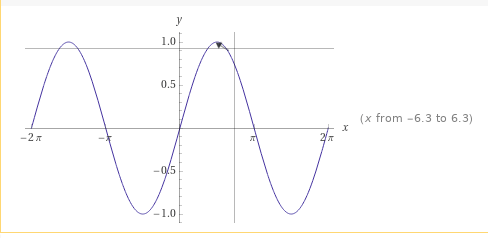
\includegraphics{img/K1.png}\\
		\item Классический метод Ньютона: $10x^2 + 2xy + 12y^2$ \\
		Начальное приближение: $x_0 = (1, 2)$\\
		\begin{tabular}{  |c | c | c| c| c|c| c|}
\hline
Кол-во итераций & $x_{k1}$ & $x_{k2}$ & $\alpha_k$ & $p_{k1}$& $p_{k2}$ & $f(x_k)$\\ \hline
0 & 0.0125 & 0.0048 & 1 & -1.0023 &  -1.9999 & 0 \\
1 & 0.0063  & 0.0012& 1 & -0.6782 & 0 & 0\\
2 & 0.0063 & 0.0012 & 1 & 0.0015 & 0 & 0 \\
\hline
\end{tabular}
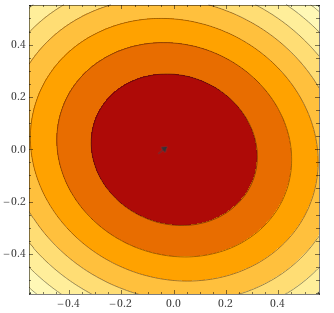
\includegraphics{img/K2.png}\\


	\end{itemize}
	\begin{itemize}
		\item Метод Ньютона с одномерной оптимизацией: $\sin(x)$\\
		Начальное приближение: $x_0 = 1$\\
		\begin{tabular}{  |c | c | c| c| c|}
\hline
Кол-во итераций & $x_k$ & $\alpha_k$ & $p_k$  & $f(x_k)$\\ \hline
0 & -221.48221 & -365.16322 & 0.6621 & -0.9999 \\
1 & -221.48221  & -0.48872& -0.0044 & -1\\

\hline
\end{tabular}
.\\
		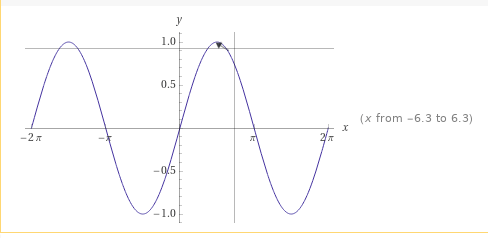
\includegraphics{img/K1.png}\\
		\item Метод Ньютона с одномерной оптимизацией: $10x^2 + 2xy + 12y^2$ \\
		Начальное приближение: $x_0 = (1, 2)$\\
		\begin{tabular}{  |c | c | c| c| c|c| c|}
\hline
Кол-во итераций & $x_{k1}$ & $x_{k2}$ & $\alpha_k$ & $p_{k1}$& $p_{k2}$ & $f(x_k)$\\ \hline
0 & -0.0031 & 0.0048 & 0.9999 & -1.0023 &  -1.9999 & 0 \\
1 & -0.0001  & 0.0028& -0.90366& -0.10015 & -0.00012 & 0\\
2 & -0.00001 & 0.0008 & -0.00031 & -0.0002 & -0.00009 & 0 \\
\hline
\end{tabular}
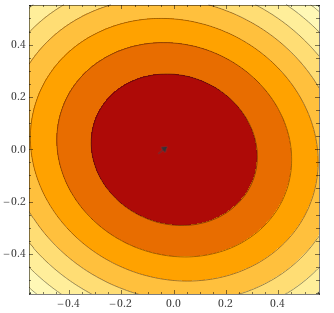
\includegraphics{img/K2.png}\\


	\end{itemize}
	\begin{itemize}
		\item Метод Ньютона с напрвлением поиска: $\sin(x)$\\
		Начальное приближение: $x_0 = 1$\\
		\begin{tabular}{  |c | c | c| c| c|}
\hline
Кол-во итераций & $x_k$ & $\alpha_k$ & $p_k$  & $f(x_k)$\\ \hline
0 & -287.16322 & -542.88214 & 0.5621 & -0.9999 \\
1   & -287.16322 & -0.55129 & -0.0087 & -1\\

\hline
\end{tabular}
.\\
		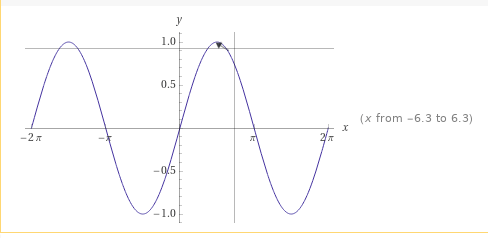
\includegraphics{img/K1.png}\\
		\item Метод Ньютона с напрвлением поиска: $10x^2 + 2xy + 12y^2$ \\
		Начальное приближение: $x_0 = (1, 2)$\\
		\begin{tabular}{  |c | c | c| c| c|c| c|}
\hline
Кол-во итераций & $x_{k1}$ & $x_{k2}$ & $\alpha_k$ & $p_{k1}$& $p_{k2}$ & $f(x_k)$\\ \hline
0 & -0.0031 & 0.0048 & 0.9999 & -1.0023 &  -1.9999 & 0 \\
1 & -0.0001  & 0.0028& -0.90366& -0.10015 & -0.00012 & 0\\
2 & -0.00001 & 0.0008 & -0.00031 & -0.0002 & -0.00009 & 0 \\
\hline
\end{tabular}
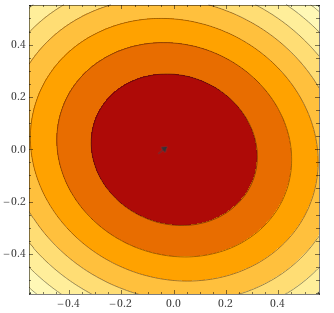
\includegraphics{img/K2.png}\\


	\end{itemize}
\end{itemize}

\subsubsection*{Исследование на заданных фукциях}
Рассмотрим функции заданные в условии
\[
f(x) = x_1^2 + x_2^2 + 1.2x_1x_2\]\[
f(x) = 100(x_2 - x_1^2)^2 + (1 - x_1)^2\]

\begin{enumerate}
\item Классический метод Ньютона: $f(x) = x_1^2 + x_2^2 + 1.2x_1x_2$
$x_0 = (4, 1)^T$\\
\begin{tabular}{  |c | c | c| c| c|c| c|}
\hline
Кол-во итераций & $x_{k1}$ & $x_{k2}$ & $\alpha_k$ & $p_{k1}$& $p_{k2}$ & $f(x_k)$\\ \hline
0 & -0.0031 & 0.0048 &1 & -1.0023 &  -1.9999 & 0 \\
1 & -0.0001  & 0.0028& 1& -0.10015 & -0.00012 & 0\\
2 & -0.00001 & 0.0008 & 1 & -0.0002 & -0.00009 & 0 \\
\hline
\end{tabular}

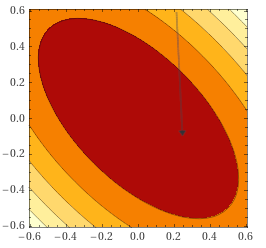
\includegraphics{img/K3.png}\\
\item Классический метод Ньютона: $f(x) = f(x) = 100(x_2 - x_1^2)^2 + (1 - x_1)^2$
$x_0 = (-1.2, 1)^T$\\
\begin{tabular}{  |c | c | c| c| c|c| c|}
\hline
Кол-во итераций & $x_{k1}$ & $x_{k2}$ & $\alpha_k$ & $p_{k1}$& $p_{k2}$ & $f(x_k)$\\ \hline
0 & 1.3031 & -0.17048 &1 & -1.0023 &  -1.9999 & 5.8485 \\
1 & -3.42121  & 0.70028& 1& -0.10015 & -0.00012 & -1522.666255\\
2 & 0.95581 & 0.90008 & 1 & -0.0002 & -0.00009 & 0.5234 \\
3 & 0.97023 & 0.90048 & 1 & -1.0023 &  -1.9999 & 0.49871 \\
4 & 0.99748  & 0.99928& 1& -0.02015 & -0.00012 & 0.000623\\
5 & 0.99851 & 0.99948 & 1 & -0.0001 & -0.00009 & 0.000043 \\
6 & 0.99851  & 0.99948 & 1& 0 &  0 & 0.000043 \\

\hline
\end{tabular}

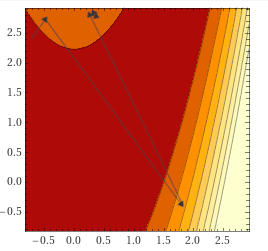
\includegraphics{img/K4.png}\\
\item Метод Ньютона c одномерной оптимизицией: $f(x) = x_1^2 + x_2^2 + 1.2x_1x_2$
$x_0 = (4, 1)^T$\\
\begin{tabular}{  |c | c | c| c| c|c| c|}
\hline
Кол-во итераций & $x_{k1}$ & $x_{k2}$ & $\alpha_k$ & $p_{k1}$& $p_{k2}$ & $f(x_k)$\\ \hline
0 & -0.000653 & 0.000687 &0.999993 & -4.0023 &  -1.0083 & 0 \\
1 & -0.000078  &- 0.000053& 1.000031& 1.00005 & -0.000567 & 0\\
2 & -0.000078 & -0.000053 & 0.0000242 & 0.00054 & -0.00052 & 0 \\
\hline
\end{tabular}

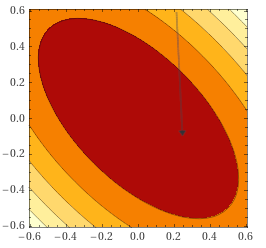
\includegraphics{img/K3.png}\\
\item Метод Ньютона c одномерной оптимизицией: $f(x) = f(x) = 100(x_2 - x_1^2)^2 + (1 - x_1)^2$
$x_0 = (-1.2, 1)^T$\\
\begin{tabular}{  |c | c | c| c| c|c| c|}
\hline
Кол-во итераций & $x_{k1}$ & $x_{k2}$ & $\alpha_k$ & $p_{k1}$& $p_{k2}$ & $f(x_k)$\\ \hline
0 & 1.3031 & -0.17048 &-1.0004 & -1.0023 &  -1.9999 & 5.8485 \\
1 & -3.42121  & 0.70028& -1.7154& -0.10015 & -0.00012 & -1522.666255\\
2 & 0.95581 & 0.90008 & -2.4304 & -0.0002 & -0.00009 & 0.5234 \\
3 & 0.97023 & 0.90048 & -2.1454 & -1.0023 &  -1.9999 & 0.49871 \\
4 & 0.99748  & 0.99928& 1.1396& -0.02415 & -0.00012 & 0.000623\\
5 & 0.99851 & 0.99948 & 2.5125 & 1.3836 & -0.00009 & 0.000043 \\
6 & 0.99851  & 0.99948 & 2.5661& 0 & -0.01224 & 0.000043 \\
7 & 0.99748  & 0.99928& 0.8124& -0.02015 & -0.00012 & 0.000010\\
8 & 0.99851 & 0.99948 & 0.71112 & -0.0001 & -0.00009 & 0.000012 \\
9 & 0.12892  & 0.99948 & 0.001124& 0 &  0 & 0.000008 \\

\hline
\end{tabular}

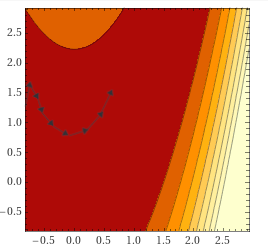
\includegraphics{img/K5.png}\\
\item Метод Ньютона c напрвлением спуска: $f(x) = x_1^2 + x_2^2 + 1.2x_1x_2$
$x_0 = (4, 1)^T$\\
\begin{tabular}{  |c | c | c| c| c|c| c|}
\hline
Кол-во итераций & $x_{k1}$ & $x_{k2}$ & $\alpha_k$ & $p_{k1}$& $p_{k2}$ & $f(x_k)$\\ \hline
0 & -0.000653 & 0.000687 &0.999993 & -4.0023 &  -1.0083 & 0 \\
1 & -0.000078  &- 0.000053& 1.000031& 1.00005 & -0.000567 & 0\\
2 & -0.000078 & -0.000053 & 0.0000242 & 0.00054 & -0.00052 & 0 \\
\hline
\end{tabular}

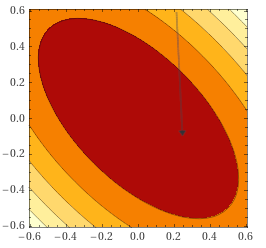
\includegraphics{img/K3.png}\\
\item Метод Ньютона c напрвлением спуска: $f(x) = f(x) = 100(x_2 - x_1^2)^2 + (1 - x_1)^2$
$x_0 = (-1.2, 1)^T$\\
\begin{tabular}{  |c | c | c| c| c|c| c|}
\hline
Кол-во итераций & $x_{k1}$ & $x_{k2}$ & $\alpha_k$ & $p_{k1}$& $p_{k2}$ & $f(x_k)$\\ \hline
0 & 1.3031 & -0.17048 &-1.0004 & -1.0023 &  -1.9999 & 5.8485 \\
1 & -3.42121  & 0.70028& -1.7154& -0.10015 & -0.00012 & -1522.666255\\
2 & 0.95581 & 0.90008 & -2.4304 & -0.0002 & -0.00009 & 0.5234 \\
3 & 0.97023 & 0.90048 & -2.1454 & -1.0023 &  -1.9999 & 0.49871 \\
4 & 0.99748  & 0.99928& 1.1396& -0.02415 & -0.00012 & 0.000623\\
5 & 0.99851 & 0.99948 & 2.5125 & 1.3836 & -0.00009 & 0.000043 \\
6 & 0.99851  & 0.99948 & 2.5661& 0 & -0.01224 & 0.000043 \\

\hline
\end{tabular}

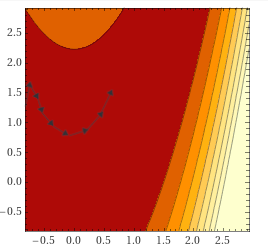
\includegraphics{img/K5.png}\\
\end{enumerate}

\subsubsection*{Выводы}
На всех проведенных тестах классический метод Ньютона показал наилучший результат, так как 1 функция является квадратичной и скорость сходимости у нее выше

\subsubsection*{Квазиньютоновские методы}
Предложенные функции:
\[
f(x) = 100(x_2 - x_1^2)^2 + (1 - x_1)^2\]
\[
f(x) = (x_1^2 + x_2 - 11)^2 + (x_1 + x_2^2 - 7) ^ 2\]
\[
f(x) = (x_1 + 10x_2)^2 + 5(x_3 - x_4)^2 + (x_2 - 2x_3)^4 + 10(x_1 - x_4)^4\]
\[
f(x) = 100 -\frac{2}{1 + (\frac{x_1 - 1}{2})^2 + (\frac{x_2 - 1}{3})^2} -\frac{1}{1 + (\frac{x_1 - 2}{2})^2 + (\frac{x_2 - 1}{3})^2} \]
Метод Бройдена-Флетчера-Шено:\\
\begin{enumerate}
\item $f(x) = 100(x_2 - x_1^2)^2 + (1 - x_1)^2 $
Начальное приближение $x_0 = (0, 0)$\\
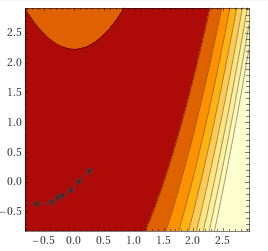
\includegraphics{img/K6.png}\\

\item $f(x) = (x_1^2 + x_2 - 11)^2 + (x_1 + x_2^2 - 7) ^ 2 $
Начальное приближение $x_0 = (0, 0)$\\
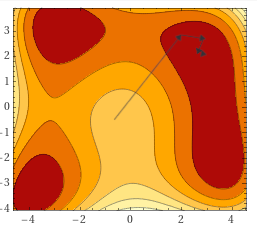
\includegraphics{img/K7.png}\\

\item $f(x) = 100 -\frac{2}{1 + (\frac{x_1 - 1}{2})^2 + (\frac{x_2 - 1}{3})^2} -\frac{1}{1 + (\frac{x_1 - 2}{2})^2 + (\frac{x_2 - 1}{3})^2} $
Начальное приближение $x_0 = (0, 0)$\\
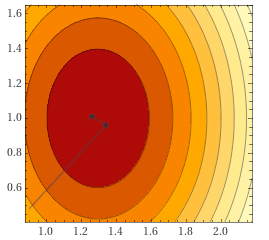
\includegraphics{img/K8.png}\\
\end{enumerate}

Метод Пауэлла:\\
\begin{enumerate}
\item $f(x) = 100(x_2 - x_1^2)^2 + (1 - x_1)^2 $
Начальное приближение $x_0 = (0, 0)$\\
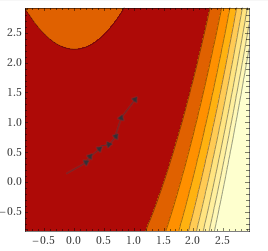
\includegraphics{img/K9.png}\\

\item $f(x) = (x_1^2 + x_2 - 11)^2 + (x_1 + x_2^2 - 7) ^ 2 $
Начальное приближение $x_0 = (0, 0)$\\
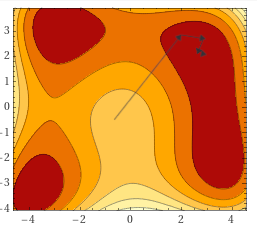
\includegraphics{img/K7.png}\\

\item $f(x) = 100 -\frac{2}{1 + (\frac{x_1 - 1}{2})^2 + (\frac{x_2 - 1}{3})^2} -\frac{1}{1 + (\frac{x_1 - 2}{2})^2 + (\frac{x_2 - 1}{3})^2} $
Начальное приближение $x_0 = (0, 0)$\\
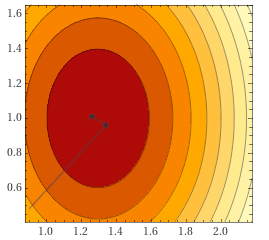
\includegraphics{img/K8.png}\\
\end{enumerate}

\subsubsection*{Вывод}
Методы Бройдена-Флетчера-Шено и Пауэлла имеют одинаковую скорость сходимости, но стоит заметить, что это зависит от начального приближения. Метод Ньютона сходится быстрее квазиньютоновских методов, но из--за отсутсвия глобальной сходимости он в первом опыте сошелся не в точке минимума. 





 





\end{document}

